\documentclass[a4paper,12pt]{jarticle}
\usepackage[dvipdfmx]{graphicx}
\usepackage{amsmath}
\usepackage{subfigure}
\usepackage{comment}

\setlength{\hoffset}{0cm}
\setlength{\oddsidemargin}{-3mm}
\setlength{\evensidemargin}{-3cm}
\setlength{\marginparsep}{0cm}
\setlength{\marginparwidth}{0cm}
\setlength{\textheight}{24.7cm}
\setlength{\textwidth}{17cm}
\setlength{\topmargin}{-45pt}

\renewcommand{\baselinestretch}{1.6}
\renewcommand{\floatpagefraction}{1}
\renewcommand{\topfraction}{1}
\renewcommand{\bottomfraction}{1}
\renewcommand{\textfraction}{0}
\renewcommand{\labelenumi}{(\arabic{enumi})}
%\renewcommand{\figurename}{Fig.} %図をFig.にする


%図のキャプションからコロン:を消す
\makeatletter
\long\def\@makecaption#1#2{% #1=図表番号、#2=キャプション本文
\sbox\@tempboxa{#1. #2}
\ifdim \wd\@tempboxa >\hsize
#1 #2\par 
\else
\hb@xt@\hsize{\hfil\box\@tempboxa\hfil}
\fi}
\makeatother


\begin{document}
%
\title{\vspace{-30mm}知能システム学特論 \ 最終レポート\\ Hdp第2班 16344217 津上祐典\\ 2016年8月19日}
\date{}
%
%
\maketitle
%
\vspace{-30mm}
%
%%%%%%%%%%%%%%%%%%%
 \section{テーマ}
%%%%%%%%%%%%%%%%%%
Spark,Hadoopを用いた機械学習によるスパムメールの分類と画像の多クラス分類
%%%%%%%%%%%%%%%%%%%
\section{概要}
%%%%%%%%%%%%%%%%%%%
はじめに,Hadoop,Spark,機械学習の原理ついて述べ,最後に実行結果と考察を
示す.
%%%%%%%%%%%%%%%%%%%%%%%
\subsection{Hadoop}
%%%%%%%%%%%%%%%%%%%%%%%
Hadoopはビッグデータを複数のPCを用いて分散並列処理を可能にするフレームワークであ
る.ー台マスターサーバとその配下にある複数のスレーブサーバによって分散
並列処理を行う.
Hadoopは分散ファイルシステム(Hadoop Distributed File
System),並列分散処理フレームワーク(MapReduce
Framework)より構成されている.分散ファイルシステムとは複数のスレーブサーバを一つのストレー
ジとして扱うファイルシステムである.身近な例でクラウドやネットワー
クHDD(NAS)などがある.並列分散処理フレームワークでは与えられたデー
タから欲しいデータの抽出と分解するMap処理,それらのデータを集計する
Reduce処理が行われる.MapReduce処理を複数のスレーブサーバで行うことで分
散処理を可能にし,ビッグデータを効率よく扱うことができる.
%
\begin{figure}[htbp]
 \begin{center}
  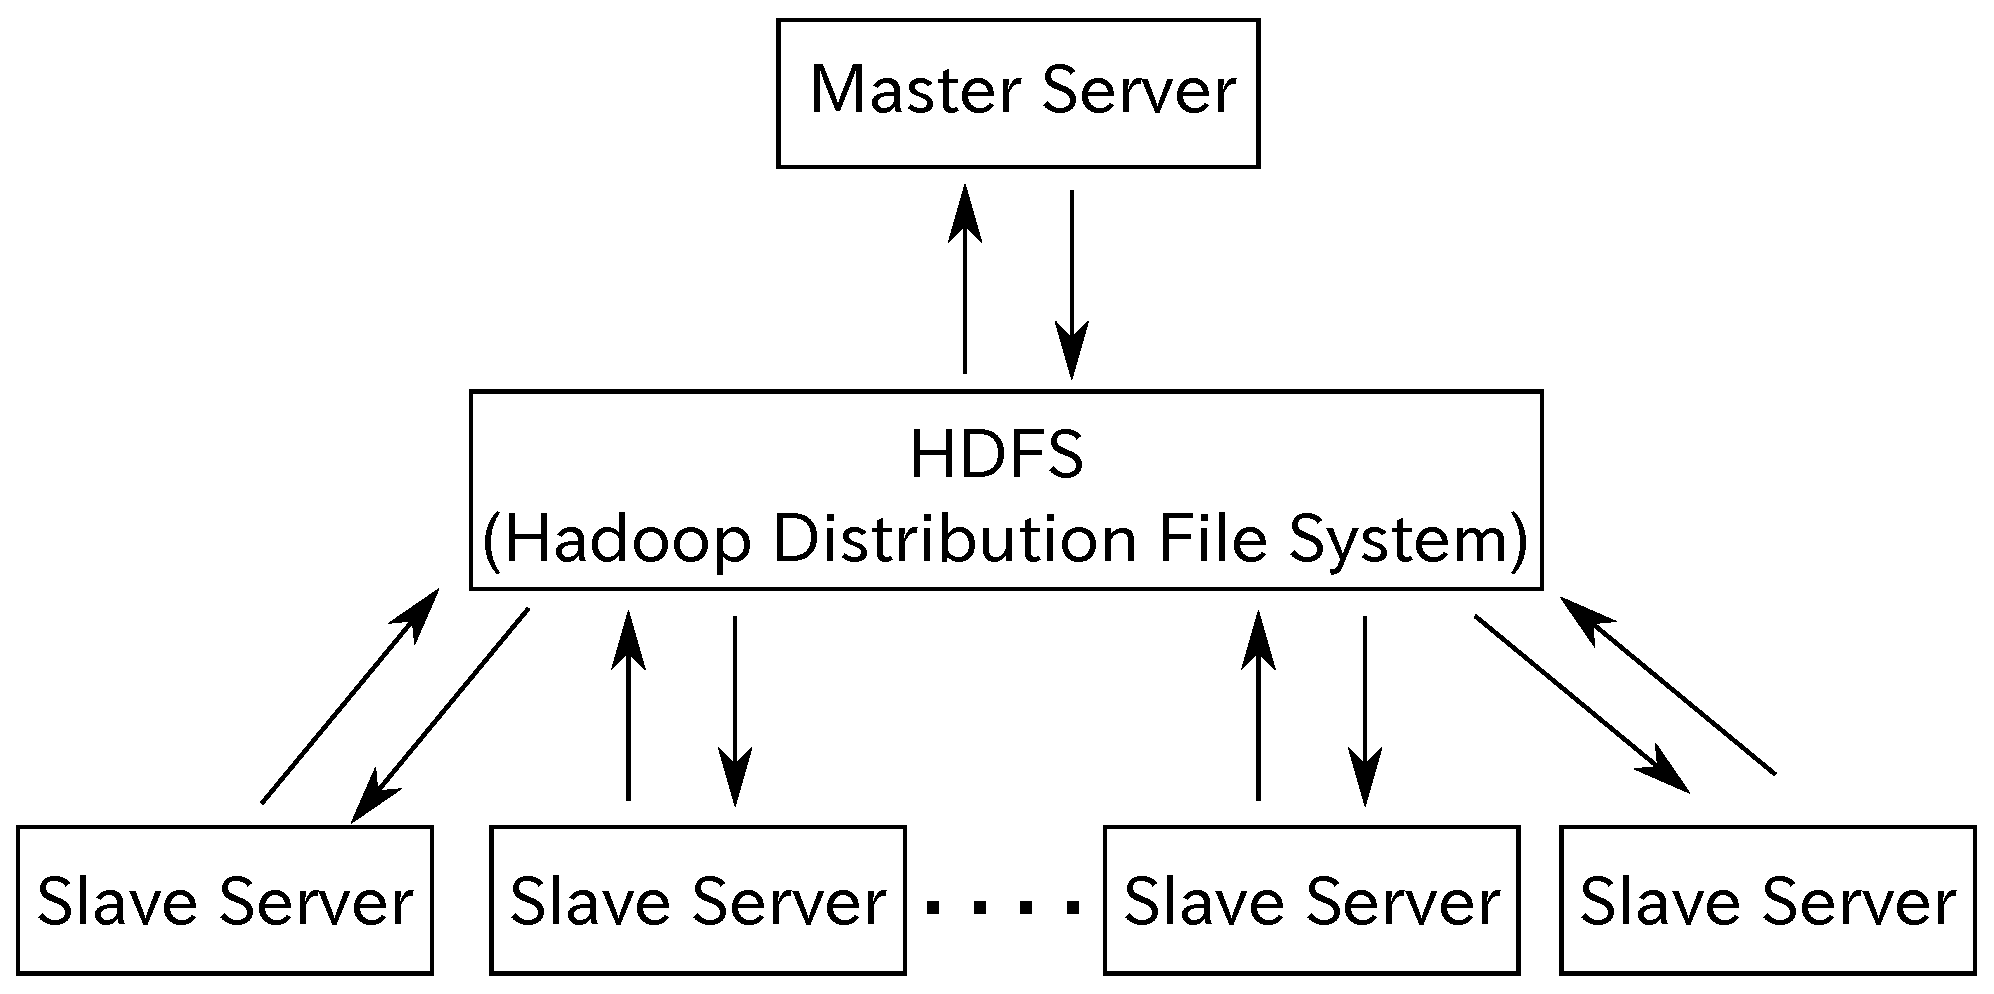
\includegraphics[width=100mm]{fig/Hadoop.eps}
  \caption{Hadoopの構成}
  \label{fig:hadoop}
 \end{center}
\end{figure}
%
%
\begin{figure}[htbp]
 \begin{center}
  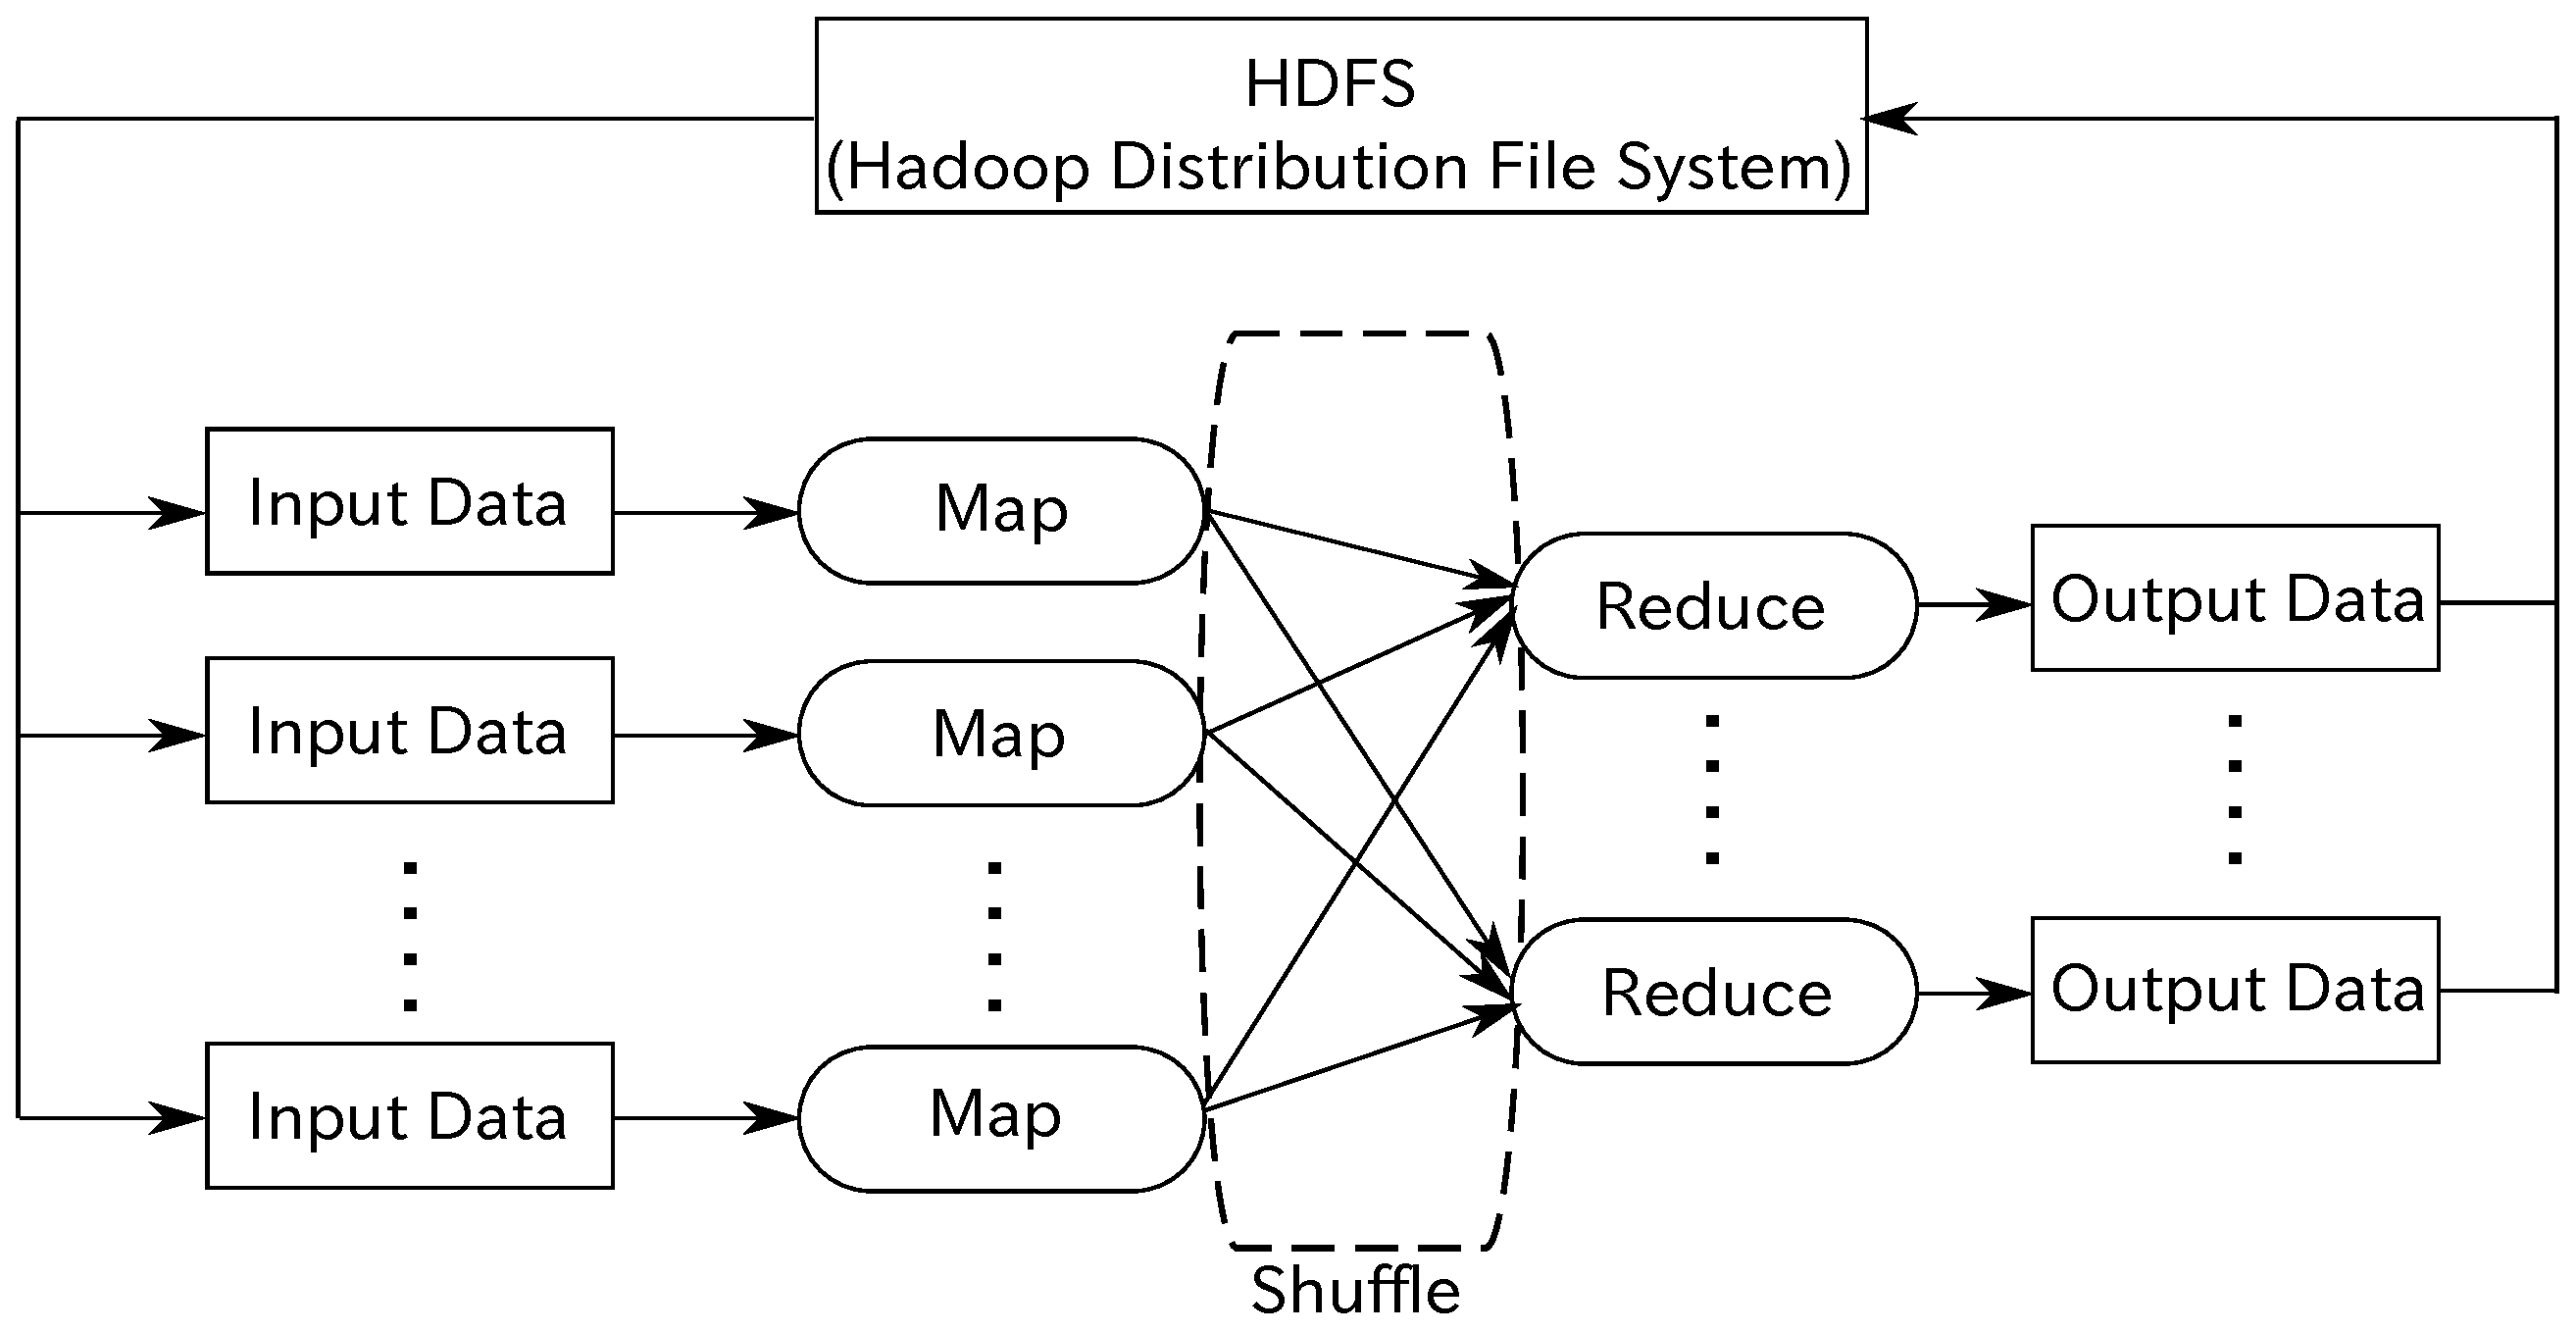
\includegraphics[width=100mm]{fig/MapReduce.eps}
  \caption{Hadoopの分散処理の流れ}
  \label{fig:MapReduce}
 \end{center}
\end{figure}
%
Hadoopは分散並列処理システムであり,Hadoopのみでは機械学習が行えない.し
かし,機械学習するためのライブラリ等のツールがいくつか用意されている.
Hdp第2班では,Sparkを用いた.次節にて,Sparkについて説明する.
%%%%%%%%%%%%%%%%%%%%%%
\subsection{Spark}
%%%%%%%%%%%%%%%%%%%%%%
SparkとはHadoop同様,分散並列処理を可能にするフレームワークである.Spark
自身はHDFSを持っておらず,HadoopのHDFSを利用することが出来る.Sparkでは
機械学習用ライブラリMLlibが用意されており,機械学習の分散並列処理が可能
である.使用可能な言語はJava,Python,R言語である.Hadoopは一つの処理が
終わるたびにHDFSに書き込まなければならないが,Sparkではインメモリに書き
込むことで,一つの処理ごとにHDFSに書き込む必要が無く,繰り返し処理に強
い特長がある.また,機械学習用のライブラリとしてMLlibが用意されている.
SparkはRDD(Resillient Distributed Datasets)


%
% \begin{figure}
 % \begin{center}
  % \subfigure[Hadoop]{%
   %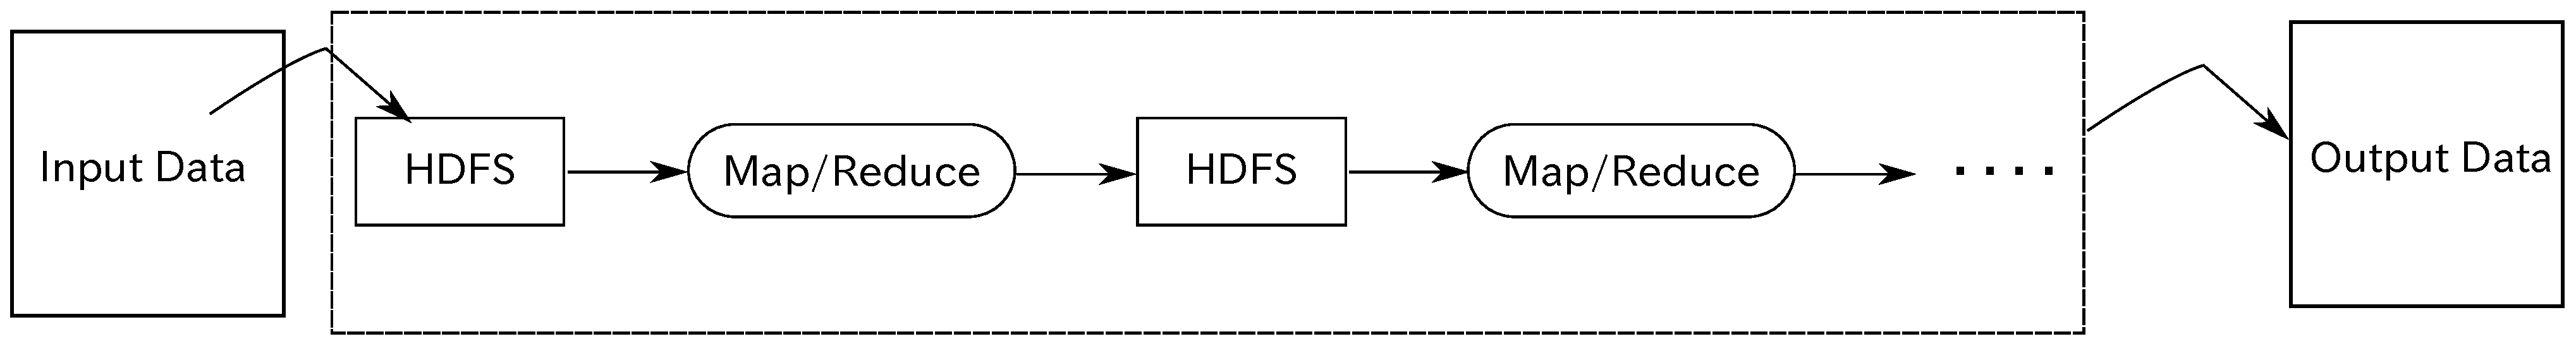
\includegraphics[width=170mm]{fig/Hadoop_d.eps}}%
   %\\
   %\subfigure[Spark]{%
   %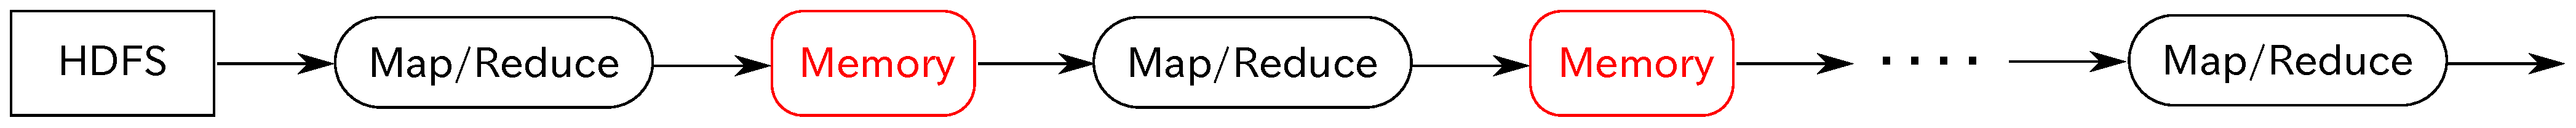
\includegraphics[width=170mm]{fig/Spark_d.eps}}%
  %\end{center}
  %\caption{HadoopとSparkの違い}
  %\label{fig:Hadoop_vs_Spark}
 %\end{figure}
%
%%%%%%%%%%%%%%%%%%%%
\subsection{機械学習(Machine Learning)}
%%%%%%%%%%%%%%%%%%%%

%%%%%%%%%%%%%%%%%%%%%%%%%%%%%%%%
\subsubsection{スパムメールの分類}
%%%%%%%%%%%%%%%%%%%%%%%%%%%%%%%%
一つ目の学習テーマとしてスパムメールの分類を行った.データセットとして
Spambase DataSet\cite{Spam}を用いた.
このデータセットは4601通のメールがあり,うち1813通のスパムメールと2788通の非スパムメー
ルから構成されている.また,57次元のベクトルとして特徴量抽出済みである.
1〜48番目の要素は特定の変数名の出現頻度,49〜54番目の要素は記号文
字の出現頻度,55〜57番目の要素は,大文字の連なりの長さの平均,最長,
合計である.学習アルゴリズムとして,ロジスティック回帰を使用した.
ロジスティック回帰とは,識別関数としてシグモイド関数を用いた回帰モデルであ
る.シグモイド関数は以下の式で表される.また,図\ref{fig:sigmoid}にシグ
モイド関数のグラフを示す.
%
\begin{equation}
 f_\theta (x) = \frac{1}{1+e^{-\theta x}}
\end{equation}
%
\begin{figure}[htbp]
 \begin{center}
  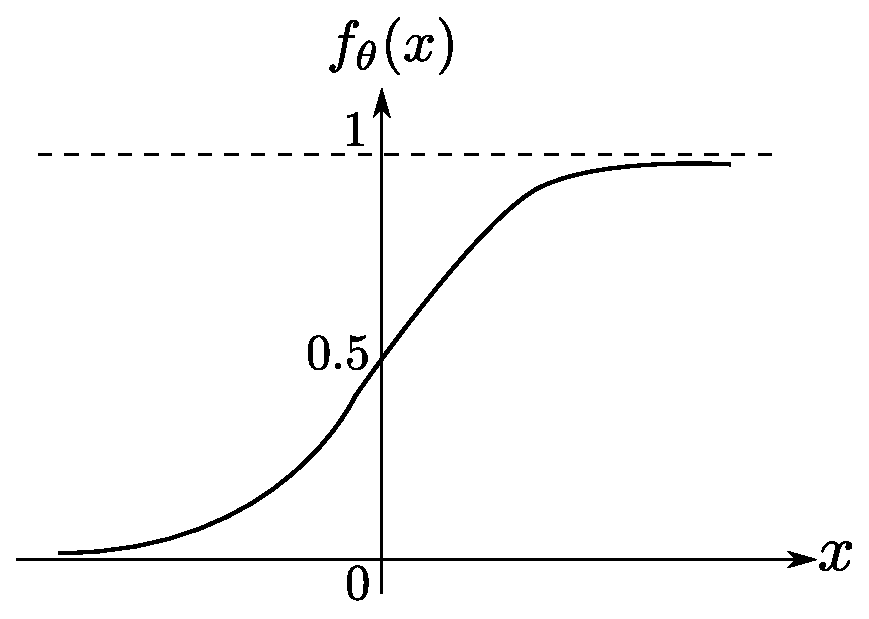
\includegraphics[width=60mm]{fig/sigmoid.eps}
  \caption{シグモイド関数}
  \label{fig:sigmoid}
 \end{center}
\end{figure}
%
ただし,$\theta$はパラメータである.目的関数である対数尤度関数$\log L(\theta)$
%
\begin{equation}
 \log L(\theta) = \sum^n_{i=1}(y^{(i)}\log f_\theta(x)+(1-y^{(i)})\log
  (1-f_\theta (x)))
\end{equation}
%
を最大化するするようなパラメータ$\theta$を学習(更新)する.パラメータの
更新式を求めるには,最急降下法や確率的勾配法,準ニュートン法などがあるが,
SparkのMLlibで用意されている準ニュートン法を用いてパラメータを更新した.


%%%%%%%%%%%%%%%%%%%%%%%%%%%%%%%%%%%%%%
\subsubsection{画像の分類}
%%%%%%%%%%%%%%%%%%%%%%%%%%%%%%%%%%%%%%
二つ目の学習テーマとして画像の分類を行った.データセットとしてCIFAR-10\cite{CIFAR}を
用いた.CIFAR-10は60000枚の画像からなり,うち50000枚が訓練用画
像であり,残り10000枚はテスト用画像である.

%%%%%%%%%%%%%%%%%
\subsection{実験}
%%%%%%%%%%%%%%%%%
その結果を表\ref{tab:実験
結果}に示す.また,ロジスティック回帰モデルで設定パラメータを実
験的にチューニングして求めた際の結果を表\ref{tab:パラメータのチューニング前後の比較}に示
す.

%%%%%%%%%%%%%%%%%%%%%%%%
\subsubsection{実行条件}
%%%%%%%%%%%%%%%%%%%%%%%%

\begin{table}[hbtp]
\centering
\caption{実行条件}
\label{tab:実行条件}
\fontsize{9pt}{10pt}\selectfont
 \begin{tabular}{|c||c|c|} \hline
 テーマ &スパムメールの検出& 画像の分類\\ \hline \hline
データセット& Spambase Data Set& CIFAR-10\\ \hline
  学習アルゴリズム& \multicolumn{2}{|c|}{ロジスティック回帰}\\ \hline
  評価法&\multicolumn{2}{|c|}{ホールドアウト法}\\ \hline
  環境&\multicolumn{2}{|c|}{Master:1台,Slave:2台}\\ \hline
  OS&\multicolumn{2}{|c|}{Ubuntu 14.04 LTS}\\ \hline
\end{tabular}
\end{table}

\begin{table}[hbt]
\centering
\caption{実験結果}
\label{tab:実験結果}
\fontsize{9pt}{10pt}\selectfont
\begin{tabular}{|c|c|c|c|c|c|} \hline
 &非スパム再現率&スパム再現率&非スパム適合率&スパム適合率&AUC(PR) \\ \hline
SVM& 76.13\%& 85.79\%& 88.90\%& 70.61\% & 0.8105 \\ \hline
ロジスティック回帰&91.92\% & 90.41\% & 93.48\% & 88.21\% & 0.9123 \\ \hline
ナイーブベイズ& 83.85\% & 66.25\% & 78.79\%  & 73.28\% & 0.7652  \\ \hline
\end{tabular}
\end{table}

\begin{table}[hbt]
\centering
\caption{パラメータのチューニング前後の比較}
\label{tab:パラメータのチューニング前後の比較}
\fontsize{9pt}{10pt}\selectfont
\begin{tabular}{|c|c|c|} \hline
 &チューニング前&チューニング後 \\ \hline
正則化関数& L2ノルム & L1ノルム \\ \hline
正則化係数&0.01 & 0.002 \\ \hline
学習繰り返し回数  &10 & 25  \\ \hline \hline
非スパム再現率& 88.60\%& 91.92\% \\ \hline
スパム再現率& 88.81\%& 90.41\% \\ \hline
非スパム適合率& 92.21\%& 93.48\% \\ \hline
スパム適合率& 83.89\%& 88.21\% \\ \hline
ACU(PR)& 0.8859 &0.9123 \\ \hline
\end{tabular}
\end{table}

%%%%%%%%%%%%%%%%%%%
\section{自分の分担範囲}
%%%%%%%%%%%%%%%%%%
機械学習・分散処理(Hadoop,Spark)の理論調査,毎週のレポート作成
%%%%%%%%%%%%%%%%%%%
\section{感想}
%%%%%%%%%%%%%%%%%%

%%%%%%%%%%%%%%%%%%%
\section{評価}
%%%%%%%%%%%%%%%%%%
\begin{table}[hbtp]
\centering
\caption{評価}
\label{tab:評価}
\fontsize{9pt}{10pt}\selectfont
\begin{tabular}{c|c||c} \hline
 学籍番号&氏名     &評価   \\ \hline \hline
16344201&井上 聖也& うわああああああああああああああああああああああああ
		 ああああああああああああああああ    \\ \hline
16344216&田中 良道& 0.002 \\ \hline
16344217&津上 祐典& 25    \\ \hline 
15344229&沈 歩偉 & 91.92 \\ \hline
\end{tabular}
\end{table}

\newpage
%参考文献
\begin{thebibliography}{99}
\addcontentsline{toc}{section}{参考文献}

 \bibitem{Spam} "Spambase Data Set",
		 https://archive.ics.uci.edu/ml/datasets/Spambase, 2016年8月9日最終確認.

 \bibitem{CIFAR} "The CIFAR-10 dataset",
		 https://www.cs.toronto.edu/~kriz/cifar.html, 2016年8月9日最終確認.

\end{thebibliography}

\end{document}
